\documentclass[11pt]{article}

\usepackage[T2A]{fontenc}
\usepackage[utf8]{inputenc}
\usepackage[russian]{babel}

\usepackage{hyphenat}
\hyphenation{ма-те-ма-ти-ка вос-ста-нав-ли-вать}

\usepackage[a4paper,margin=2cm]{geometry}

\usepackage{graphicx}
\usepackage[intlimits]{amsmath}
\usepackage{amssymb}
\usepackage{amsmath}
\usepackage{subcaption}
\usepackage{wrapfig}
\usepackage{float}
\usepackage{fancyhdr}
\usepackage{mathtools}
\usepackage{tensor}
\usepackage{pgf}
\usepackage{array}
\usepackage[utf8]{inputenc}\DeclareUnicodeCharacter{2212}{-}

\newcommand{\rot}[1]{[\nabla, \mathbf{#1}]}
\newcommand{\di}[1]{(\nabla, \mathbf{#1})}
\newcommand{\ve}[1]{\mathbf{#1}}
\newcommand{\re}[1]{(\ref{#1})}


\begin{document}
 Задача: решить задачу Коши системы обыкновенных дифференциальных уравнений: \\
 \[
  \begin{dcases} 
   \frac{dy_1}{dx} = -49y_1 + 125y_2, \\
   \frac{dy_2}{dx} = 20y_1 - 49y_2.
  \end{dcases}
  ;
  \begin{dcases}
   y_1(0) = A, \\
   y_2(0) = B.
  \end{dcases}
  ;
  0 < x < D = 1.
\]

 Сначала построим аналитическое решение задачи(просто потому что можем):\\
\[
\frac{d}{dx}
 \begin{pmatrix}
  y_1 \\
  y_2
 \end{pmatrix}
 =
 \begin{pmatrix}
  -49 & 125 \\
  20 & -49
 \end{pmatrix}
 \begin{pmatrix}
  y_1 \\
  y_2
 \end{pmatrix}
\]
Ищем собственные значения и собственные вектора матрицы:
\[
 \begin{vmatrix}
  -49 - \lambda & 125 \\
  20 & -49 - \lambda
 \end{vmatrix}
 =
 (49 + \lambda)^2 - 2500 = 0 \Rightarrow \lambda_{1,2} = 1, -99.
\]
Откуда $\ve{h_1} = (5, 2)^T $; $\ve{h_2} = (5, -2)^T$. \\
Общее решение системы запишется в виде:
\[
 \begin{pmatrix}
  y_1 \\
  y_2
 \end{pmatrix}
  =
  C_1 \ve{h_1} e^x + C_2 \ve{h_2} e^{-99x}.
\]
С учетом граничных условий:
\[
 \begin{pmatrix}
  y_1 \\
  y_2
 \end{pmatrix}
 =
 \left(\frac{A}{10} - \frac{B}{4}\right)\cdot
 \begin{pmatrix}
   5 \\
   -2
 \end{pmatrix}
 e^{-99x}
 + 
 \left(\frac{A}{10} + \frac{B}{4}\right)
 \begin{pmatrix}
  5 \\
  2
 \end{pmatrix}
 e^{x}.
\]
Теперь о численном методе. Я использовал классический метод Рунге-Кутты 4-го порядка. Он задается таблицей Бутчера: \\
\begin{tabular}{c | c c c c}
0 & 0 & 0 & 0 & 0 \\
1/2 & 1/2 & 0 & 0 & 0 \\
1/2 & 0 & 1/2 & 0 & 0 \\
1 & 0 & 0 & 1 & 0 \\ \hline
 & 1/6 & 1/3 & 1/3 & 1/6 
\end{tabular} 

Видно, что для этого метода выполняются соотношения Кутты:
\[
 c_j = \sum^s_{k=1} a_{jk},
\]
а потому условия аппроксимации имеют вид:\\
для 1-го порядка:
\[
 \sum^{s}_{j=1}b_j = \frac{1}{6} + \frac{2}{6} + \frac{2}{6} + \frac{1}{6} = 1
\]
для второго:
\[
 \sum^s_{j=1}b_jc_j = \frac{1}{6} + \frac{1}{6} + \frac{1}{6} = \frac{1}{2}
\]
для третьего:
\[
 \sum^s_{j=1}b_jc^2_j = \frac{1}{12} + \frac{1}{12} + \frac{1}{6} = \frac{1}{3}
\]
\[
 \sum^s_{j=1}\sum^s_{k=1} b_ja_{jk}c_k = \frac{1}{12} + \frac{1}{12} = \frac{1}{6}
\]
для четвертого:
\[
 \sum^s_{j=1}b_jc_j^3 = \frac{1}{24} + \frac{1}{24} + \frac{1}{6} = \frac{1}{4}
\]
\[
 \sum^s_{j=1}\sum^s_{k=1}b_ja_{jk}c_jc_k = \frac{1}{24} + \frac{1}{12} = \frac{1}{8}
\]
\[
 \sum^s_{j=1}\sum^s_{k=1}b_ja_{jk}c^2_k = \frac{1}{24} + \frac{1}{24} = \frac{1}{12}
\]
\[
 \sum^s_{j=1}\sum^s_{k=1}\sum^s_{l=1}b_ja_{jk}a_{kl}c_l = \frac{1}{24} = \frac{1}{24}
\]
Видно, что все они выполняются.\\
Метод явный, 4-х стадийный, с 4 порядком аппроксимации, поэтому функция устойчивости для него имеет вид:
\[
 1 + z + \frac{z^2}{2} + \frac{z^3}{6} + \frac{z^4}{24}.
\]
Область устойчивости выглядит так:
\begin{figure}[H]
\centering
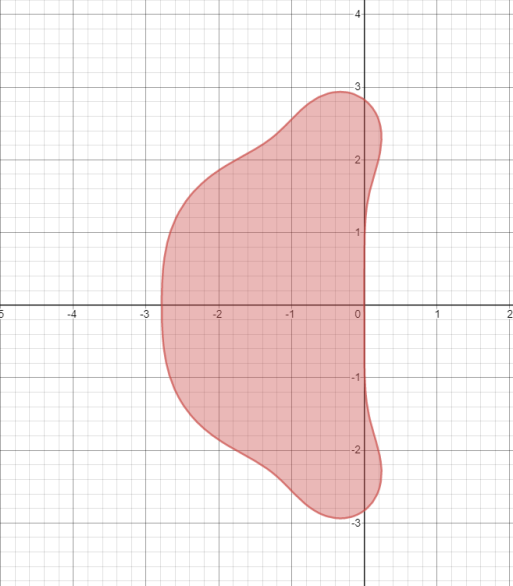
\includegraphics[width=0.45\linewidth]{ust_001.png}
\end{figure}
То есть на действительной оси $-2.7855 < z < 0$. \\
$z = \lambda h$, откуда зная наши $\lambda$ найдем $h$. В этой задаче метод устойчив при $h \le 0.02814$. \\
Здесь и далее --- результаты вычислений на сетках с последовательно уменьшающимся шагом. Для определенности выбраны А = 1, В = 1.\\

h = 0.1 \\ 
\begin{tabular}{c | c c c c c c c}
$i$ & $x_i$ & $y_1(x_i)$ & $[y_1]_{x_i}$ & $|[y_1]_{x_i} - y_1(x_i)|$ & $y_2(x_i)$ & $[y_2]_{x_i}$ & $|[y_2]_{x_i} - y_2(x_i)|$ \\ \hline
1 & 0.1 & -207.043579 & 1.93401148 & 208.977591 & 84.3646708 & 0.773634695 & 83.5910361 \\
2 & 0.2 & -58226.728 & 2.13745482 & 58228.8654 & 23292.4011 & 0.854981931 & 23291.5462 \\
3 & 0.3 & -16224704.5 & 2.36225291 & 16224706.9 & 6489883.71 & 0.944901165 & 6489882.76 \\
4 & 0.4 & -4.52080102e+09 & 2.61069322 & 4.52080102e+09 & 1.80832041e+09 & 1.04427729 & 1.80832041e+09 \\
5 & 0.5 & -1.2596617e+12 & 2.88526222 & 1.2596617e+12 & 5.0386468e+11 & 1.15410489 & 5.0386468e+11 \\
6 & 0.6 & -3.50988152e+14 & 3.1887079 & 3.50988152e+14 & 1.40395261e+14 & 1.27548316 & 1.40395261e+14 \\
7 & 0.7 & -9.77982288e+16 & 3.52406724 & 9.77982288e+16 & 3.91192915e+16 & 1.4096269 & 3.91192915e+16 \\
8 & 0.8 & -2.72501892e+19 & 3.89469662 & 2.72501892e+19 & 1.09000757e+19 & 1.55787865 & 1.09000757e+19 \\
\end{tabular} \newpage

h = 0.05 \\ 
\begin{tabular}{c | c c c c c c c}
$i$ & $x_i$ & $y_1(x_i)$ & $[y_1]_{x_i}$ & $|[y_1]_{x_i} - y_1(x_i)|$ & $y_2(x_i)$ & $[y_2]_{x_i}$ & $|[y_2]_{x_i} - y_2(x_i)|$ \\ \hline
2 & 0.1 & -126.816853 & 1.93401148 & 128.750865 & 52.2739806 & 0.773634695 & 51.500346 \\
4 & 0.2 & -22100.2557 & 2.13745482 & 22102.3932 & 8841.81226 & 0.854981931 & 8840.95728 \\
6 & 0.3 & -3794268.4 & 2.36225291 & 3794270.76 & 1517709.25 & 0.944901165 & 1517708.31 \\
8 & 0.4 & -651354378 & 2.61069322 & 651354380 & 260541753 & 1.04427729 & 260541752 \\
10 & 0.5 & -1.11816619e+11 & 2.88526222 & 1.11816619e+11 & 4.47266476e+10 & 1.15410489 & 4.47266476e+10 \\
12 & 0.6 & -1.91953208e+13 & 3.1887079 & 1.91953208e+13 & 7.67812833e+12 & 1.27548316 & 7.67812833e+12 \\
14 & 0.7 & -3.29521984e+15 & 3.52406724 & 3.29521984e+15 & 1.31808794e+15 & 1.4096269 & 1.31808794e+15 \\
16 & 0.8 & -5.65683372e+17 & 3.89469662 & 5.65683372e+17 & 2.26273349e+17 & 1.55787865 & 2.26273349e+17 \\
18 & 0.9 & -9.71096595e+19 & 4.30430544 & 9.71096595e+19 & 3.88438638e+19 & 1.72172218 & 3.88438638e+19 \\
\end{tabular}

h = 0.025 \\ 
\begin{tabular}{c | c c c c c c c}
$i$ & $x_i$ & $y_1(x_i)$ & $[y_1]_{x_i}$ & $|[y_1]_{x_i} - y_1(x_i)|$ & $y_2(x_i)$ & $[y_2]_{x_i}$ & $|[y_2]_{x_i} - y_2(x_i)|$ \\ \hline
4 & 0.1 & 1.82000154 & 1.93401148 & 0.11400994 & 0.819238671 & 0.773634695 & 0.0456039755 \\
8 & 0.2 & 2.12011236 & 2.13745482 & 0.0173424639 & 0.861918916 & 0.854981931 & 0.00693698447 \\
12 & 0.3 & 2.35961576 & 2.36225291 & 0.00263715684 & 0.945956026 & 0.944901165 & 0.00105486093 \\
16 & 0.4 & 2.6102922 & 2.61069322 & 0.000401018092 & 1.04443769 & 1.04427729 & 0.000160404573 \\
20 & 0.5 & 2.88520124 & 2.88526222 & 6.09842785e-05 & 1.15412928 & 1.15410489 & 2.4390032e-05 \\
24 & 0.6 & 3.18869862 & 3.1887079 & 9.27887859e-06 & 1.27548687 & 1.27548316 & 3.70667177e-06 \\
28 & 0.7 & 3.52406582 & 3.52406724 & 1.41791514e-06 & 1.40962746 & 1.4096269 & 5.60874389e-07 \\
32 & 0.8 & 3.8946964 & 3.89469662 & 2.24350502e-07 & 1.55787873 & 1.55787865 & 8.17934953e-08 \\
36 & 0.9 & 4.3043054 & 4.30430544 & 4.49553506e-08 & 1.72172219 & 1.72172218 & 8.1018614e-09 \\
\end{tabular}

h = 0.0125 \\ 
\begin{tabular}{c | c c c c c c c}
$i$ & $x_i$ & $y_1(x_i)$ & $[y_1]_{x_i}$ & $|[y_1]_{x_i} - y_1(x_i)|$ & $y_2(x_i)$ & $[y_2]_{x_i}$ & $|[y_2]_{x_i} - y_2(x_i)|$ \\ \hline
8 & 0.1 & 1.93398503 & 1.93401148 & 2.64473016e-05 & 0.773645274 & 0.773634695 & 1.05788895e-05 \\
16 & 0.2 & 2.13745482 & 2.13745482 & 3.67264885e-09 & 0.854981933 & 0.854981931 & 1.40020207e-09 \\
24 & 0.3 & 2.36225291 & 2.36225291 & 1.43058898e-10 & 0.944901165 & 0.944901165 & 5.69250203e-11 \\
32 & 0.4 & 2.61069322 & 2.61069322 & 2.10256257e-10 & 1.04427729 & 1.04427729 & 8.41029468e-11 \\
40 & 0.5 & 2.88526222 & 2.88526222 & 2.904601e-10 & 1.15410489 & 1.15410489 & 1.16184173e-10 \\
48 & 0.6 & 3.1887079 & 3.1887079 & 3.85209198e-10 & 1.27548316 & 1.27548316 & 1.54084301e-10 \\
56 & 0.7 & 3.52406724 & 3.52406724 & 4.9667559e-10 & 1.4096269 & 1.4096269 & 1.98670191e-10 \\
64 & 0.8 & 3.89469662 & 3.89469662 & 6.27327523e-10 & 1.55787865 & 1.55787865 & 2.50931276e-10 \\
72 & 0.9 & 4.30430544 & 4.30430544 & 7.79971643e-10 & 1.72172218 & 1.72172218 & 3.11988213e-10 \\
\end{tabular}

h = 0.00625 \\ 
\begin{tabular}{c | c c c c c c c}
$i$ & $x_i$ & $y_1(x_i)$ & $[y_1]_{x_i}$ & $|[y_1]_{x_i} - y_1(x_i)|$ & $y_2(x_i)$ & $[y_2]_{x_i}$ & $|[y_2]_{x_i} - y_2(x_i)|$ \\ \hline
16 & 0.1 & 1.9340107 & 1.93401148 & 7.72196416e-07 & 0.773635004 & 0.773634695 & 3.08876611e-07 \\
32 & 0.2 & 2.13745482 & 2.13745482 & 8.36917202e-11 & 0.854981931 & 0.854981931 & 2.91509039e-11 \\
48 & 0.3 & 2.36225291 & 2.36225291 & 8.97015795e-12 & 0.944901165 & 0.944901165 & 3.58313379e-12 \\
64 & 0.4 & 2.61069322 & 2.61069322 & 1.32081013e-11 & 1.04427729 & 1.04427729 & 5.28377342e-12 \\
80 & 0.5 & 2.88526222 & 2.88526222 & 1.82454052e-11 & 1.15410489 & 1.15410489 & 7.29838412e-12 \\
96 & 0.6 & 3.1887079 & 3.1887079 & 2.41966447e-11 & 1.27548316 & 1.27548316 & 9.67914637e-12 \\
112 & 0.7 & 3.52406724 & 3.52406724 & 3.11990433e-11 & 1.4096269 & 1.4096269 & 1.24795729e-11 \\
128 & 0.8 & 3.89469662 & 3.89469662 & 3.94058119e-11 & 1.55787865 & 1.55787865 & 1.57625024e-11 \\
144 & 0.9 & 4.30430544 & 4.30430544 & 4.89981389e-11 & 1.72172218 & 1.72172218 & 1.95989891e-11 \\
\end{tabular}

h = 0.003125 \\ 
\begin{tabular}{c | c c c c c c c}
$i$ & $x_i$ & $y_1(x_i)$ & $[y_1]_{x_i}$ & $|[y_1]_{x_i} - y_1(x_i)|$ & $y_2(x_i)$ & $[y_2]_{x_i}$ & $|[y_2]_{x_i} - y_2(x_i)|$ \\ \hline
32 & 0.1 & 1.93401144 & 1.93401148 & 3.68498603e-08 & 0.77363471 & 0.773634695 & 1.4739823e-08 \\
64 & 0.2 & 2.13745482 & 2.13745482 & 4.03899136e-12 & 0.854981931 & 0.854981931 & 1.34448008e-12 \\
96 & 0.3 & 2.36225291 & 2.36225291 & 5.61328761e-13 & 0.944901165 & 0.944901165 & 2.24043006e-13 \\
128 & 0.4 & 2.61069322 & 2.61069322 & 8.26894109e-13 & 1.04427729 & 1.04427729 & 3.31290551e-13 \\
160 & 0.5 & 2.88526222 & 2.88526222 & 1.139977e-12 & 1.15410489 & 1.15410489 & 4.56301663e-13 \\
192 & 0.6 & 3.1887079 & 3.1887079 & 1.51079149e-12 & 1.27548316 & 1.27548316 & 6.04849504e-13 \\
224 & 0.7 & 3.52406724 & 3.52406724 & 1.94821936e-12 & 1.4096269 & 1.4096269 & 7.79376563e-13 \\
256 & 0.8 & 3.89469662 & 3.89469662 & 2.46158649e-12 & 1.55787865 & 1.55787865 & 9.84767823e-13 \\
288 & 0.9 & 4.30430544 & 4.30430544 & 3.06421555e-12 & 1.72172218 & 1.72172218 & 1.22524213e-12 \\
\end{tabular}

h = 0.0015625 \\ 
\begin{tabular}{c | c c c c c c c}
$i$ & $x_i$ & $y_1(x_i)$ & $[y_1]_{x_i}$ & $|[y_1]_{x_i} - y_1(x_i)|$ & $y_2(x_i)$ & $[y_2]_{x_i}$ & $|[y_2]_{x_i} - y_2(x_i)|$ \\ \hline
64 & 0.1 & 1.93401147 & 1.93401148 & 2.01547246e-09 & 0.773634696 & 0.773634695 & 8.06182676e-10 \\
128 & 0.2 & 2.13745482 & 2.13745482 & 2.22488694e-13 & 0.854981931 & 0.854981931 & 7.28306304e-14 \\
192 & 0.3 & 2.36225291 & 2.36225291 & 3.37507799e-14 & 0.944901165 & 0.944901165 & 1.3211654e-14 \\
256 & 0.4 & 2.61069322 & 2.61069322 & 4.97379915e-14 & 1.04427729 & 1.04427729 & 2.04281037e-14 \\
320 & 0.5 & 2.88526222 & 2.88526222 & 6.75015599e-14 & 1.15410489 & 1.15410489 & 2.68673972e-14 \\
384 & 0.6 & 3.1887079 & 3.1887079 & 8.83737528e-14 & 1.27548316 & 1.27548316 & 3.5971226e-14 \\
448 & 0.7 & 3.52406724 & 3.52406724 & 1.14130927e-13 & 1.4096269 & 1.4096269 & 4.57411886e-14 \\
512 & 0.8 & 3.89469662 & 3.89469662 & 1.44328993e-13 & 1.55787865 & 1.55787865 & 5.77315973e-14 \\
576 & 0.9 & 4.30430544 & 4.30430544 & 1.82964754e-13 & 1.72172218 & 1.72172218 & 7.3052675e-14 \\
\end{tabular}

h = 0.00078125 \\ 
\begin{tabular}{c | c c c c c c c}
$i$ & $x_i$ & $y_1(x_i)$ & $[y_1]_{x_i}$ & $|[y_1]_{x_i} - y_1(x_i)|$ & $y_2(x_i)$ & $[y_2]_{x_i}$ & $|[y_2]_{x_i} - y_2(x_i)|$ \\ \hline
128 & 0.1 & 1.93401148 & 1.93401148 & 1.1132717e-10 & 0.773634695 & 0.773634695 & 4.45321557e-11 \\
256 & 0.2 & 2.13745482 & 2.13745482 & 1.15463195e-14 & 0.854981931 & 0.854981931 & 4.6629367e-15 \\
384 & 0.3 & 2.36225291 & 2.36225291 & 0 & 0.944901165 & 0.944901165 & 4.4408921e-16 \\
512 & 0.4 & 2.61069322 & 2.61069322 & 8.8817842e-16 & 1.04427729 & 1.04427729 & 4.4408921e-16 \\
640 & 0.5 & 2.88526222 & 2.88526222 & 4.4408921e-16 & 1.15410489 & 1.15410489 & 2.22044605e-16 \\
768 & 0.6 & 3.1887079 & 3.1887079 & 1.33226763e-15 & 1.27548316 & 1.27548316 & 8.8817842e-16 \\
896 & 0.7 & 3.52406724 & 3.52406724 & 1.77635684e-15 & 1.4096269 & 1.4096269 & 6.66133815e-16 \\
1024 & 0.8 & 3.89469662 & 3.89469662 & 1.77635684e-15 & 1.55787865 & 1.55787865 & 6.66133815e-16 \\
1152 & 0.9 & 4.30430544 & 4.30430544 & 8.8817842e-16 & 1.72172218 & 1.72172218 & 8.8817842e-16 \\
\end{tabular}

Видно, что пока мы не достигли рассчитаного значения $h$, необходимого для устойчивости, погрешность была большой. Однако затем решение к чему-то сошлось. Для демонстрации --- сравнение с графиком аналитического решения.
\begin{figure}[H]
\centering
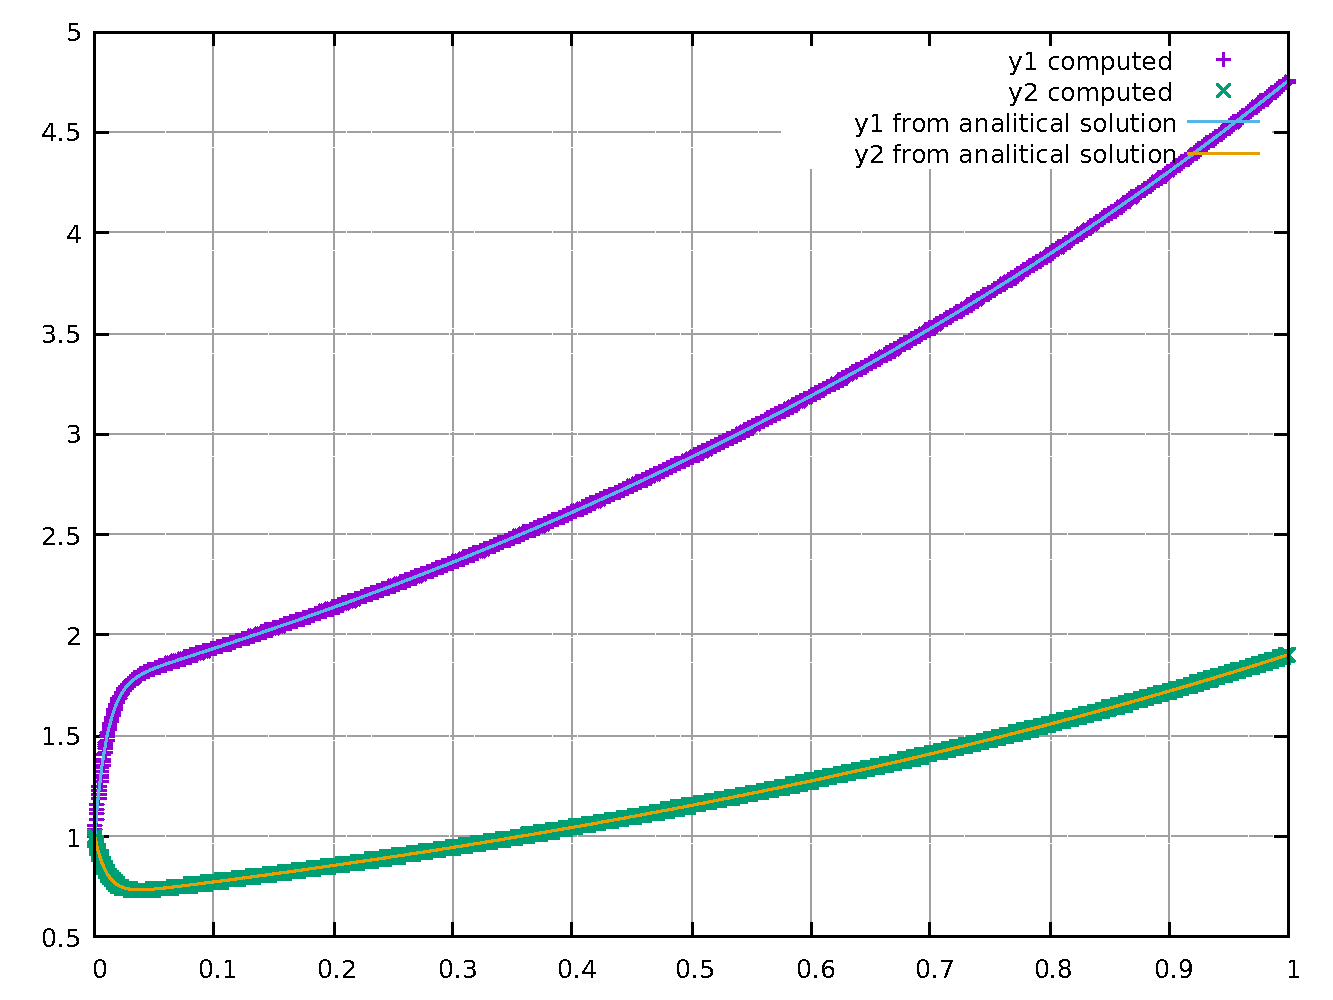
\includegraphics[width=0.65\linewidth]{graph.pdf}
\end{figure}





 
\end{document}
